% (C) Copyright 2016
% Urs Fässler, www.bitzgi.ch
% SPDX-License-Identifier: CC-BY-SA-4.0

\section{Vorstellung}
\begin{frame}{About me}
	\begin{center}
		\begin{tikzpicture}
		[
			node distance = 3 cm,
			box/.style = {align=center},
		]
		
		\visible<1-> {
			\node[box] (me) {\large{Urs Fässler}};
		}
		
		\visible<2-> {
			\node[box, above left of = me] {
\includegraphics[height=1cm]{res/fellowship-page-logo.pdf}};
		}
	
		\visible<3-> {
			\node[box, above right of = me] {
\includegraphics[height=1cm]{res/bbv.pdf}};
		}
	
		\visible<4-> {
			\node[box, below right of = me] {
\includegraphics[height=1.5cm]{res/cpp.pdf}};
		}
	
		\visible<5-> {
			\node[box, below left of = me] {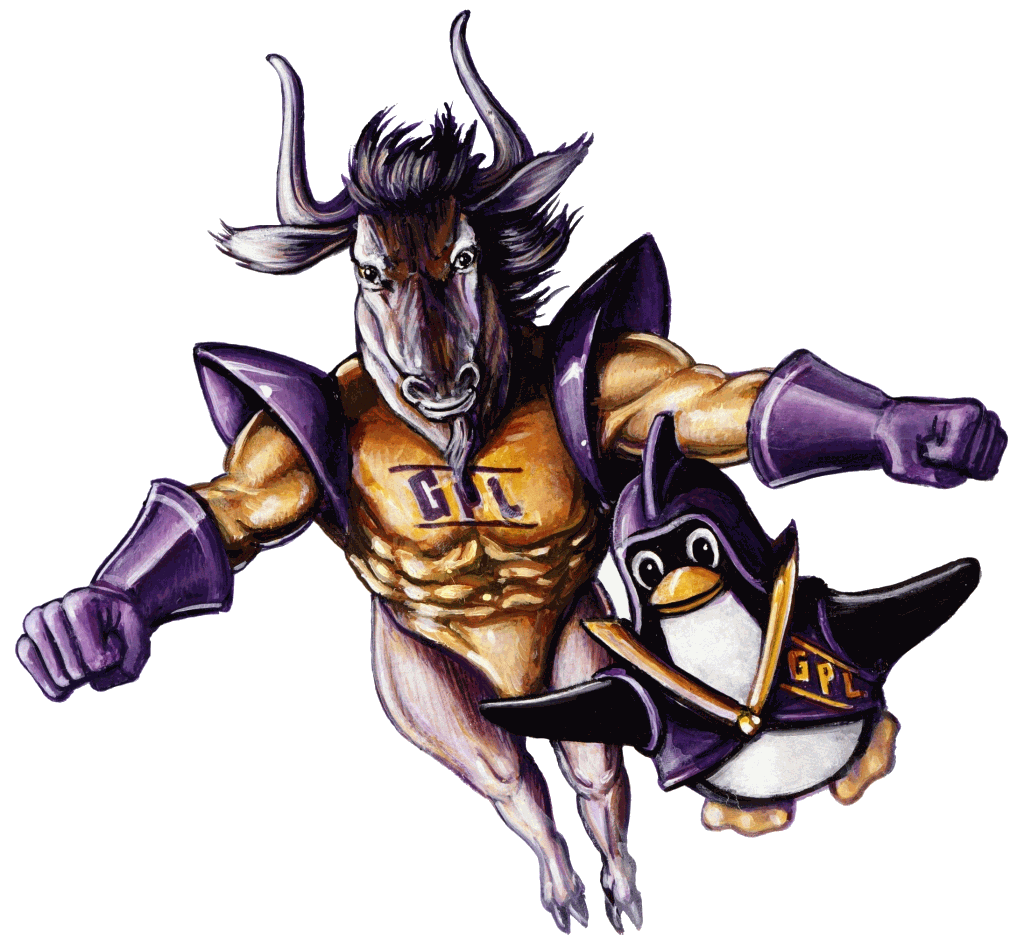
\includegraphics[height=4cm]{res/gnu-and-penguin-color.png}};
		}
	
		\end{tikzpicture}
	\end{center}
\end{frame}
\note
{
	\begin{itemize}
		\item Urs Fässler
		\item Aktiv in der FSFE Lokalgruppe Zürich
		\item Senior Embedded Software Ingenieur @ bbv Software Service \url{http://bbv.ch}
		\item Entwickeln von Software
		\item Erstellen von Systemen auf Basis GNU/Linux
		\item FSFE Fellow: \url{https://fsfe.org/contribute/getyourgraphic.en.html}
		\item Gnu-and-penguin-color.png: GFDL 1.2+ or CC-BY-SA 3.0 (\url{https://commons.wikimedia.org/wiki/File:Gnu-and-penguin-color.png})
	\end{itemize}
}

\begin{frame}{Haftungsausschluss}
	\begin{itemize}
		\item Dieser Vortrag ist keine Rechtsberatung.
		\item Für eine Rechtsberatung konsultieren Sie bitte einen Anwalt.
	\end{itemize}
\end{frame}
